% File SDSS2020_SampleExtendedAbstract.tex
\documentclass[11pt]{article}
\usepackage{sdss2020} % Uses Times Roman font (either newtx or times package)
\usepackage{url}
\usepackage{latexsym}
\usepackage{amsmath, amsthm, amsfonts}
\usepackage{algorithm, algorithmic}
\usepackage{graphicx}
\usepackage{adjustbox}
\usepackage{setspace}
\setstretch{1}
\graphicspath{{images/}}

\title{Artificial Neural Networks and Deep Learning \\
Homework 2}

\author{
  Nicola Dean \\
  10674826 \\
  {\tt nicola.dean \\
  \tt @mail.polimi.it} \\\And
  Marco Fasanella \\
  10617541 \\
  {\tt marco.fasanella \\
  \tt @mail.polimi.it} \\\And
  Raffaello Fornasiere \\
    10790353 \\
    {\tt raffaello.fornasiere \\
    \tt @mail.polimi.it} \\\And
  Christian Spano \\
  10823764 \\
  {\tt christian.spano \\
  \tt @mail.polimi.it} \\}


\date{}

\begin{document}
\maketitle


\section{Introduction}
In this homework our approach has been to predict the target variables at a future time point based on the learning from previous time points.\\
To keep the problem tractable, learning methods used  use data from a fixed length window in the past as an explicit input.\
the range of possible solutions was limited compared to the previous task, in this case the tests done included RNN, Resnet, LSTM and 1D CNN models.\\
In order to ease the development of our best solution, we thought it would have been useful to create an ad-hoc helper.\\
As a matter of fact, a lot of code is often repeated or many lines of code are needed just to plot or to get insightful results (such as the confusion matrix or the accuracy).
In particular it has been useful to build sequences and data augmentation (dealing with randomness and noise).
\section{Vanilla Models}
We first approached a Vanilla model in order to understand if we could easily tackle the classification problem with a 1D Convolutional Neuronal Network.\\
The best configuration we found consisted in 3 convolutions followed by a Dropout and 2 Dense layers:

This model unfortunately arrived at a result of maximum 0.70 in terms of local Accuracy, reached with a grid search on filters,kernels and dropout.\\
We then moved to a Vanilla LSTM and Bidirectional-LSTM, but with poor results.

\section{Preprocessing}
When it comes to TimeSeries classification/forecasting, preprocessing is a crucial step to grant optimal results.\
In this section will be described all the preprocessing techniques we tried or discarded.
\subsection{Normalization}
After visualizing the data, we noticed that samples has different scale factor based on targets.\
To avoid advantaging some of the classes we decided to normalize the dataset.
\subsubsection{Per Column}
As first approach, we normalized the dataset by \textbf{FULL columns}
\begin{itemize}
  \item \textbf{MinMax} Does not work properly; When applied, the validation accuracy dropped to 33%.
  \item \textbf{Mean / Std} This technique does not improve the accuracy on vanilla models.
\end{itemize}
\subsubsection{Per Sample}
The next method we tried, was to normalize each sample (TimeSeries) independently, to completly remove the different scales of the targets.
\begin{itemize}
  \item \textbf{MinMax} Improve performances but not enough, at least on vanilla models
  \item \textbf{Mean / Std} This was the \textbf{Game Changer} for us, it improves the performances on Vanilla models from 63\% to 67\% on the Vanilla BiLstm
\end{itemize}
\subsection{Augmentation}
In the Homework1 challenge, we noticed the importance of augmentation on this field and so we decided to give it a try also on time series.\
We tried both "by hand" and Library approach with the following results.
\subsubsection{Numpy}
Using the function \textit{np.random.normal} it is possible to generate random noise with a certain mean std and shape.\
To obtain augmented samples we copied the dataset multiple time, and then, for each time serie, we calculated it's standard deviation and applied the augmentation like follow:

\begin{figure}[h]
  \[ x = x + np.random.normal(0,std,x.shape) * w\]
  \caption{With x be a single time series, w be a weight of our choice}
\end{figure}

The result of augmentation was immediate and bring us a solid 68\% using the vanilla BiLstm (that was performing only 67\% without augmentation)
\subsubsection{TSUNG/Librery}
%Per raffaello, cambia il nome del titoletto come vuoi
 RAFFAELLO
\subsection{Seasonal + Trend preprocess}
Christian
\subsection{Expanding Window size}
\subsection{Adding New Features}
Christian

\section{Net Concatenations}
Now that our Preprocessing was giving promising results and the possible changes to vanilla models was not giving results better than 68.0\%
we decided to try combining LSTM and CNN into a single network.
\subsection{CNN + LSTM}
At first we combined an CNN with a LSTM thinking to use the CNN as feature extractor for the LSTM.
This was giving us the same results of BiLstm + Norm + Augm.
\subsection{LSTM + CNN}
We also tried using LSTM to analyze the time series and then CNN as feature extractor for the analyzed data
but the result was the same of BiLstm also in this case.

\section{Inspired By Existing Models}
\subsection{InceptionNet}
\begin{figure}[h]
\centering
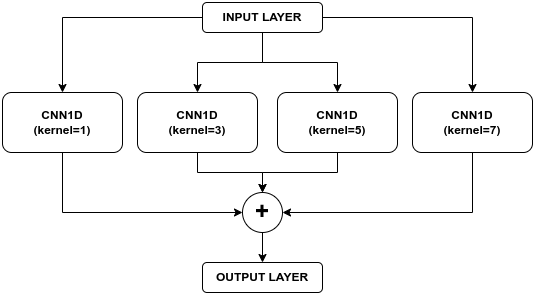
\includegraphics[width=8cm, height=4cm]{Inception}
\caption{CNN1D Inception Like Net}
\end{figure}

\subsection{Resnet}
\subsubsection{Resnet-CNN1D}
Resnet Model works by adding a big number of layer blocks alternated by some skip layers to avoid vanishing gradient descent.\
We replicated this model in keras using Conv1D instead of the original Conv2D but unfortunatly it has not improved performances and we were still stucked to 68\%.
\subsubsection{Resnet-LSTM}
A second step we had done was to replace the CNN1D with some LSTM like in figure3,
This improved the performances by 0.9\% respect to our best model so far, bringing the accuracy on codalab to 68.9\%.
\begin{figure}[h]
\centering
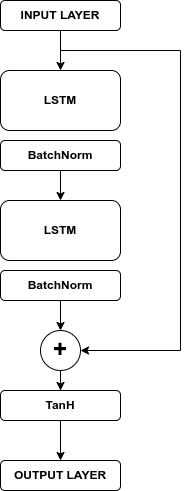
\includegraphics[width=4cm, height=8cm,angle =90]{resnet}
\caption{Resnet Like LSTM Net}
\end{figure}

\section{Heterogeneus Layers}
Not seeing results by contatenating network we thought to create a network of Hybrid layers of LSTM and CNN
\subsection{LSTM + CNN Blocks}
Not seeing results by concatenating network we thought to create a network of Hybrid layers of LSTM and CNN
\subsection{LSTM + CNN}
By inspiration on the last laboratories on Time Series forecasting, we tried to create multiple layer of LSTM + CNN
obtaining an improvement in performances from 68\% to 69\% in respect to the vanilla BiLstm.
\subsection{CNN + LSTM Blocks}
We also tried to do the opposite obtaining slightly better results (70\% on submission).
\begin{figure}[h]
  \centering
  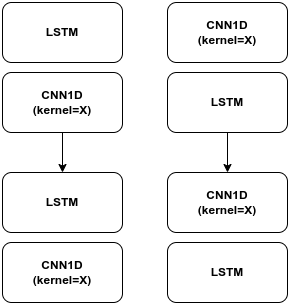
\includegraphics[width=6cm, height=5cm]{LSTMCNN}
  \caption{LSTM-CNN and CNN-LSTM Hybrid Blocks}
\end{figure}

\subsection{CNN + DENSE Blocks}
\subsection{ALTRI DI RAFFAELLO}

\section{Our best Model}
Unexpectedly bla bla bla





\section{Conclusion}

\begin{figure}[h]
  \centering
  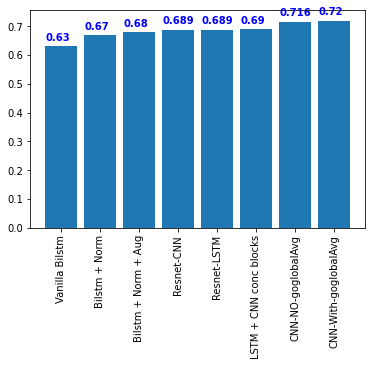
\includegraphics[width=8cm, height=6cm]{chart}
  \caption{LSTM-CNN and CNN-LSTM Hybrid Blocks}
\end{figure}

\bibliographystyle{sdss2020} % Please do not change the bibliography style
\bibliography{SampleReferencesForExtendedAbstract}

\end{document}
